\section{Tensión de entrada y salida: linealidad y limitaciones}

\subsection{Análisis teórico}

Si se pensara en un modelo completamente ideal, se esperaría que el $Op$ $Amp$ amplifique por el valor de la ganancia todas las señales que se apliquen entre sus entradas. Sin embargo, en la realidad 
se verifican limitaciones a su ganancia, dependiendo tanto de límites ya fijados para la tensión aplicada como de otros fenómenos en función de la frecuencia de la señal.

Uno de los primeros fenómenos observados es que la linealidad planteada por la relación:

$$v_{out}=A_{v}v_{d}=A_{v_{ol}}(v^{+}-v^{-})=-A_{v_{ol}}v^{-}$$ 

no se cumple para todos los valores de tensión de entrada,
sino que a partir de un valor la tensión de salida dejará de amplificar linealmente y se llegará a la \textbf{saturación}: a pesar de aumentar la magnitud de la 
señal de entrada, ésta no continúa amplificandose por encima de ese valor de saturación. Esto se debe a que las fuentes de alimentación fijan valores límites de amplificación de la señal de entrada.

Dado que la tensión de salida de un circuito equivale al producto entre la ganancia y la tensión de entrada. Modelizando la tensión mediante la ganancia ideal del operacional y reemplazando con una $Vcc = 9v$, se obtiene la siguiente expresión:

$$V_{in_{max}}=\frac{V_{cc}}{G_{ideal}}=\frac{9v}{G_{ideal}}$$

Si se considera el modelo de primer órden estudiado, la ganancia está dada por el módulo de la función transferencia, de la cual resulta que:

$$V_{in_{max}}=\frac{9v}{\left | H(s) \right |}$$

De modo que para cada circuito se tienen las siguientes expresiones:

\textbf{Inversor:}
\begin{equation} \label{eq:sat1}
    V_{in_{max}}=\frac{V_{cc}R_{1}}{R_{2}}\sqrt{(\frac{2\pi}{w_{b'}})^{2}f^{2}+(1+\frac{k}{A_{ol}})^{2}}
    k=\frac{R_{1}R_{3}+R_{1}R_{2}+R_{2}R_{3}}{R_{1}R_{3}}
\end{equation}



\textbf{No inversor:}

\begin{equation} \label{eq:sat2}
    V_{in_{max}}=\frac{V_{cc}}{A_{ol}(R_{1}+R_{2})R_{4}}\sqrt{(\frac{2\pi q_{1}}{w_{b}})^{2}f^{2}+q_{2}^{2}}
\end{equation}
\begin{equation}
\left\{\begin{matrix}
q_{1}=(R_{3}+R_{4})(R_{1}+R_{2})
\\ 
q_{2}=(R_{3}+R_{4})+(R_{2}+R_{1}+R_{1}A_{ol})
\end{matrix}\right.
\end{equation}


Sin embargo, se debe tener en cuenta que en la realidad la saturación no equivale al valor de la tensión de la fuente de alimentación, siendo menor en módulo. El valor de la tensión de saturación está detallado por la ''Oscilación de tensión de salida'', rango de valores de entrada en modo común en el cual el amplificador opera linealmente. En la hoja de datos del integrado se explicita que dicho rango corresponde a una tensión de 0 a $v^{+}$ - 1.5 V. Es decir, se espera que la saturación se produzca aproximadamente a los 7,5V.

La causa de la limitación en la señal de entrada y salida, dada para un valor menor que la tensión de alimentación, se encuentra en la estructura interna del amplificador operacional. Los transistores que constituyen el amplificador no son elementos lineales, entrando en saturación y en corte en determinadas instancias. Esto limita la amplificación de la señal de entrada. 

Otro efecto que limita la tensión de salida y atenta contra su linealidad es el efecto de \textbf{Slew Rate}. Se lo define como la máxima tasa de cambio en la tensión de salida con el cambio de en la tensión de entrada. El $slew$ $rate$ se da cuando la derivada de la señal de salida supera el valor característico del amplificados. En el caso del LM324, es $slew$ $rate$ es de alrededor $5\frac{V}{\mu s}$. 

El efecto de slew rate encuentra su raiz en la presencia del capacitor de compensación (también llamados capacitor de Miller) en la estructura interna del $Op$ $Amp$ el cual limita la velocidad a la que se propaga la señal. El capacitor de compensación es utilizado para corregir algunas características de la respuesta en frecuencia del operacional. Se visualiza en ésto la complejidad que implica el diseño del integrado. 

El $slew$ $rate$ se define matemáticamente como:

$$SR\geq max\left | \frac{dv_{out}}{dt} \right |$$

Considerando una tensión de entrada senoidal de amplitud $V_{p}$ y dado que la magnitud de la tensión de salida equivale al producto entre la ganancia y la tensión de entrada, se opera del siguiente modo:

$$v_{in}(t)=V_{p}\sin (2\pi ft)$$

$$v_{out}=\left | H(f) \right |v_{in}(t)\Rightarrow v_{out}=\left | H(f) \right |V_{p}\sin (2\pi ft)$$

Considerando la derivada de la señal de entrada y reemplazandola en la definición de SR:

$$\frac{dv_{in}}{dt} = V_{p}\cdot \cos (2\pi ft)\cdot 2\pi f $$

$$SR\geq max\left | \frac{dv_{out}}{dt} \right | = \left | H(f) \right |V_{p}\cdot 2\pi f$$

Finalmente, para evitar el efecto del $slew$ $rate$ el valor de la amplitud de la señal de entrada debe responder a la siguiente inecuación:

$$V_{p}=V_{in_{max}}<\frac{SR}{\left | H(f) \right |2\pi f}$$

Reemplazando por las ganancias de los circuitos, se obtiene el valor de la amplitud de la señal de entrada:

\textbf{Inversor:}

\begin{equation} \label{eq:sr1}
V_{in_{max}}<\frac{SR\cdot R_{1}}{2\pi f\cdot R_{2}}\sqrt{(\frac{2\pi}{w_{b'}})^{2}f^{2}+(1+\frac{k}{A_{ol}})}
\end{equation}


\textbf{No inversor:}

\begin{equation} \label{eq:sr2}
V_{in_{max}}<\frac{SR}{2\pi f\cdot A_{ol}(R_{1}+R_{2})R_{4}}\sqrt{(\frac{2\pi q_{1}}{w_{b}})^{2}f^{2}+q_{2}^{2}}
\end{equation}



Una última limitación visualizada durante las mediciones es la llamada \textbf{distorsión de cruce por cero}. Este efecto se visualiza en la señal de salida como una pequeña meseta de tensión cero, en la transición entre señales positivas y negativas. Justamente, este efecto se produce en algunos amplificadores operacionales por el retardo de transición que tienen sus transistores internos al conmutar de saturación a corte. Según se investigó, una forma de resolver esta pequeña distorsión es suministrando una pequeña tensión de $offset$ de continua. 

\begin{figure}[H]
	\centering
	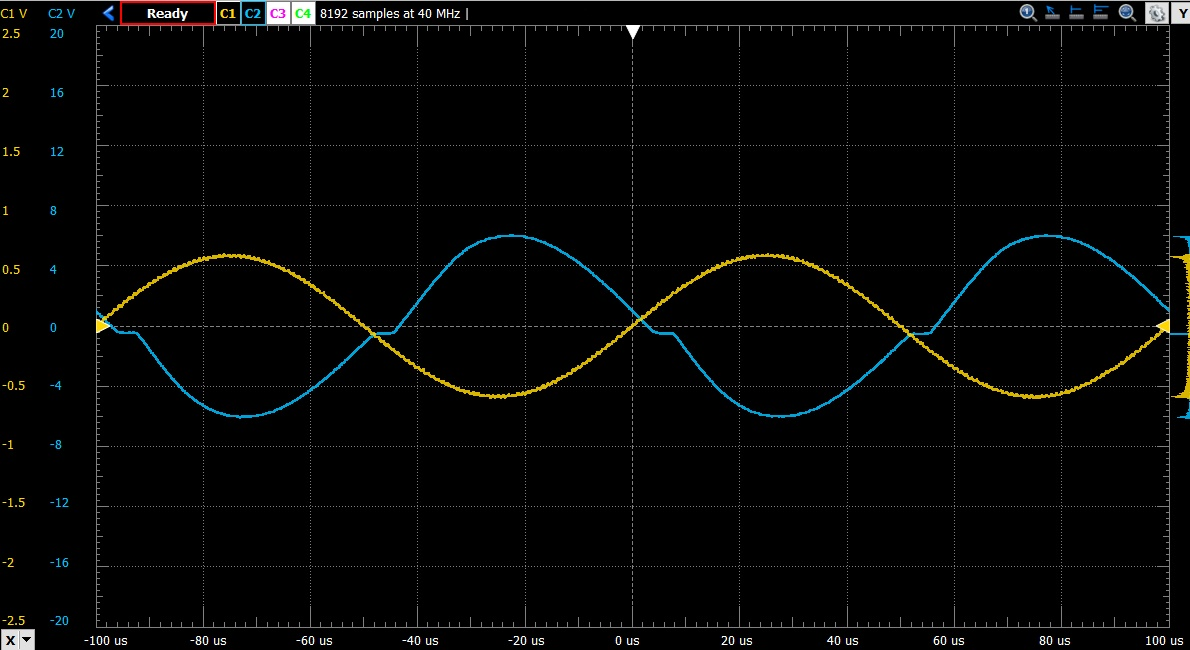
\includegraphics[scale=0.3]{./Imagenes/zeroCrossover600mV10kHz.jpg}
	\caption{Distorsión de cruce por cero. Circuito inversor caso 1 con $V_{in}$ senoidal a $10kHz$ y $1.2V_{pp}$}
	\label{fig:circinvcaso1}
\end{figure}

Seguidamente, se mostrarán ejemplos de éstas limitaciones al realizar mediciones sobre los circuitos estudiados. 

\subsection{Resultados: circuito inversor}


Para cada uno de los casos del circuito inversor, se reemplazaron los valores en las funciones \ref{eq:sat1} y \ref{eq:sr1} superponiéndolos, respectivamente. Se detallan los gráficos a continuación:


\begin{figure}[H]
	\begin{subfigure}{.5\textwidth}
	    \centering
		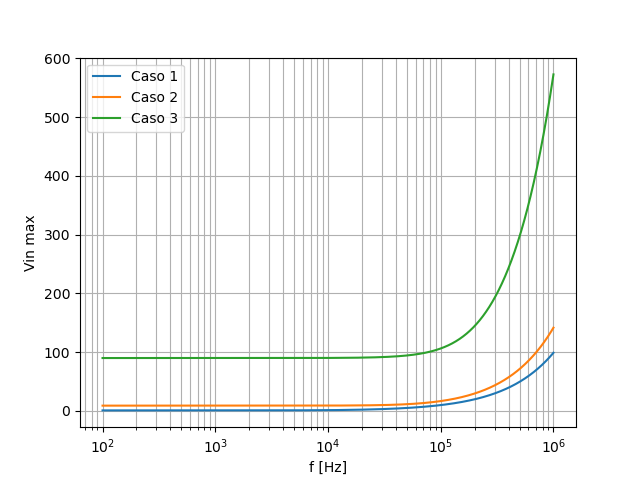
\includegraphics[width=.8\linewidth]{./Imagenes/SatInv.png}  
		\caption{Tensión de entrada limitada por efecto de saturación}
	\end{subfigure}
	\begin{subfigure}{.5\textwidth}
	    \centering
		\includegraphics[width=.8\linewidth]{./Imagenes/SRInv.png}  
		\caption{Tensión de entrada limitada por efecto de Slew Rate}
	\end{subfigure}
	\caption{Circuito inversor. Limitaciones a la tensión de entrada}
	\label{fig:invcasos}
\end{figure} 

Se puede observar que el efecto de saturación es importante a bajas frecuencias, mientras que a frecuencias altas prima la limitación a la tensión de entrada fijada por el Slew Rate.

Considerando ambos efectos, se tiene la siguiente gráfica que muestra que a altas frecuencias tensión de entrada debe ser menor a fin de mantener la linealidad con la tensión de salida. Esta disminución en la tensión de entrada a frecuencias elevadas, sumado al hecho que a frecuencias altas la ganancia es muy baja, añaden dificultad y ruido a las mediciones. 

\begin{figure}[H]
	\centering
	\includegraphics[scale=0.5]{./Imagenes/InvVinMin.png}
	\caption{Limitaciones a la tensión de entrada por saturación y slew rate}
	\label{fig:circinvcaso1}
\end{figure}

Para medir la saturación de la tensión de salida, se midió sobre el circuito y mediante simulación la tensión de salida en un rango de valores desde $-V_{cc}$ y $+V_{cc}$. Para realizar la medición, se utilizó una señal de entrada senoidal de $1kHz$ de modo de evitar los efectos antes descriptos, variando su amplitud en el rango de tensiones mencionado y relevando los datos. 

Se graficaron los resultados superpuestos con los valores teóricos de la tensión de salida, los cuales, según la teoría, son igual al los valores mínimos en valor absoluto entre la tensión $Vcc = 9V$ y el producto $G_{ideal} \cdot V_{in}$. Los resultados fueron los siguientes:

\begin{figure}[H]
	\centering
	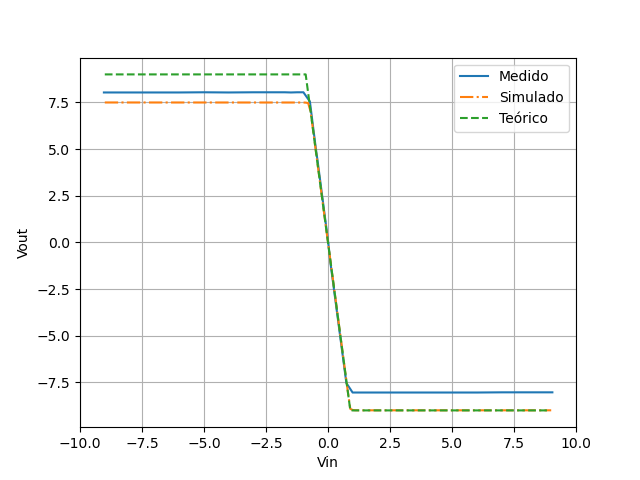
\includegraphics[scale=0.5]{./Imagenes/InvCaso1DC.png}
	\caption{DC Sweep: circuito inversor caso 1}
	\label{fig:circinvcaso1}
\end{figure}

\begin{figure}[H]
	\centering
	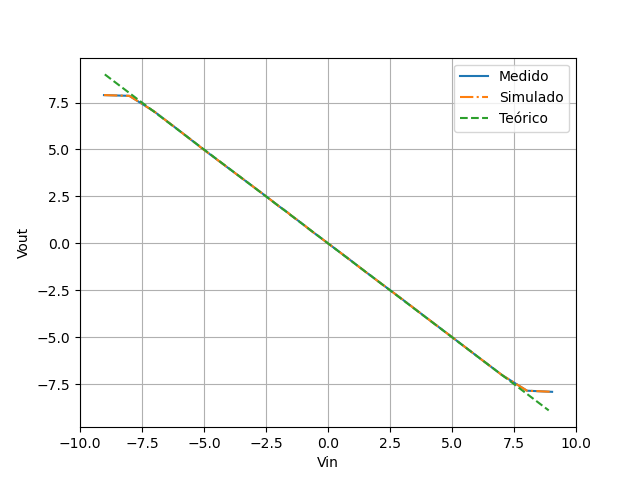
\includegraphics[scale=0.5]{./Imagenes/InvCaso2DC.png}
	\caption{DC Sweep: circuito inversor caso 2}
	\label{fig:circinvcaso1}
\end{figure}

\begin{figure}[H]
	\centering
	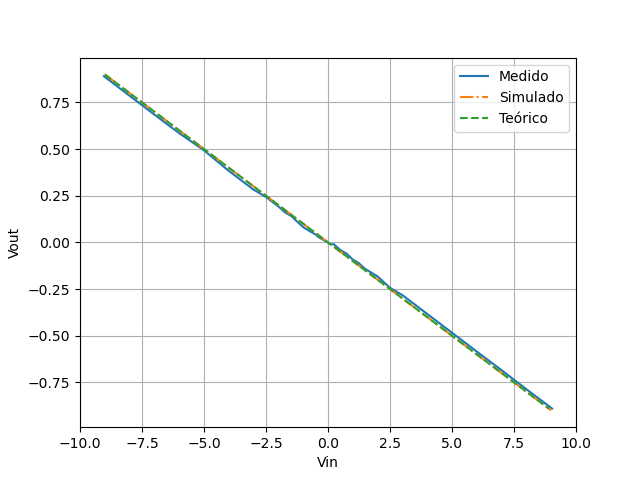
\includegraphics[scale=0.5]{./Imagenes/InvCaso3DC.png}
	\caption{DC Sweep: circuito inversor caso 3}
	\label{fig:circinvcaso1}
\end{figure}

Se observar grandes coincidencias entre los valores medidos, simulados y teóricos. Se verifica la inversión esperada en la tensión de salida. En el caso 1 y 2, además, se observa la tensión de saturación, la cual se da aproximadamente a los $7,5V$, valor presentado anteriormente. Se observa que el caso 1, el de mayor ganancia en módulo, la saturación se produce en a valores muy bajos de tensión de entrada, limitando la linealidad entre la señal de entrada y la de salida a un rango muy acotado de tensiones. Con circuitos que tengan una ganancia menor, el rango donde se presenta la linealidad entre los circuitos es mayor, tal como se observa en el caso 3 para el cual la relación entre las señales es lineal en todo el rango de trabajo. 

Para observar el efecto de \textbf{Slew Rate} se empleó el caso 1 estimulando el circuito con una señal senoidal de $2V_{pp}$ a una frecuencia de $500kHz$, observando la siguiente señal en el osciloscopio. 

\begin{figure}[H]
	\centering
	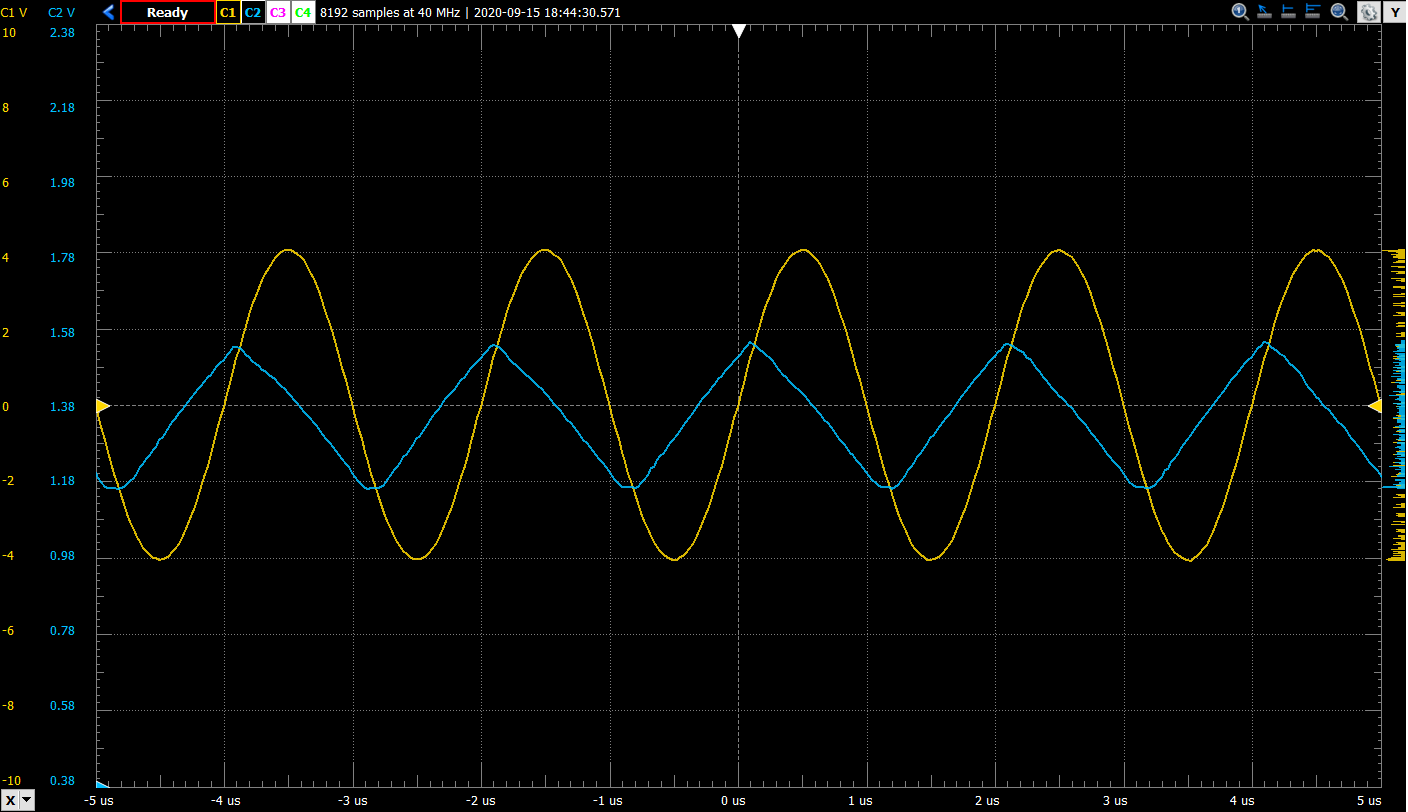
\includegraphics[scale=0.3]{./Imagenes/ICaso1SR.png}
	\caption{Slew rate: señal de entrada a $500kHz$ y $2V_{pp}$. Caso 1.}
	\label{fig:circinvcaso1}
\end{figure}

Se puede observar que la señal de salida se aproxima a una triangular, no acompañando a la señal de entrada. Para aproximar el Slew Rate que se observa se utilizó el cursor del osciloscopio estimando los valores de la pendiente, de modo que el SR observado resulta:

 $$\frac{\Delta X}{\Delta Y} \simeq \frac{0,114V}{0,875}\simeq  0,13 \frac{V}{\mu s}$$
 
Este valor de SR es bastante menor al que presenta la hoja de datos. Un SR con este valor indica que la tasa de cambio por unidad de tiempo es bastante pobre, indicando que el amplificador no es muy sensible a los cambios. Sin embargo, en las mediciones con el No Inversor se obtuvieron otros valores, por lo que podría deberse a una cuestión de medición; para futuras instancias se podría considerar medir el efecto de SR con una amplitud mayor y a una mayor frecuencia, aunque eso también implica mayor dificultad y error al ubicar los cursores sobre la imagen. 

\subsection{Resultados: circuito no inversor}

Procediendo de la misma forma que en el circuito inversor, se reemplazaron los valores en las funciones \ref{eq:sat2} y \ref{eq:sr2}, superponiendo los casos en las respectivas gráficos. 

Se obtienen las mismas conclusiones que para el circuito inversor; esto es, a altas frecuencias la principal limitación se da por slew rate mientras que a bajas frecuencias se debe prestar atención a la saturación de la señal de salida. 

\begin{figure}[H]
	\begin{subfigure}{.5\textwidth}
	    \centering
		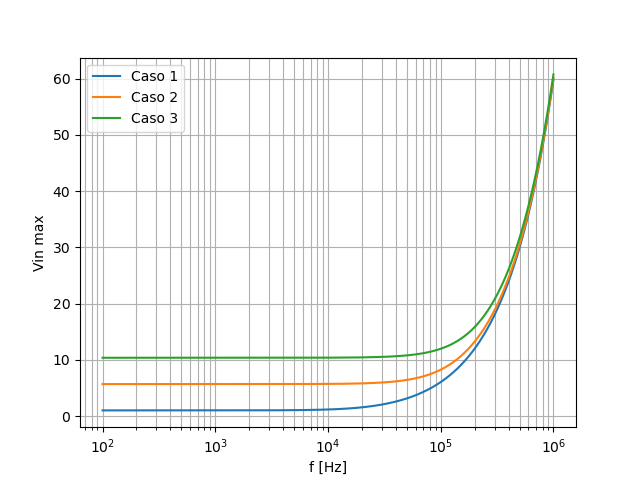
\includegraphics[width=.8\linewidth]{./Imagenes/SatNoInv.png}  
		\caption{Tensión de entrada limitada por efecto de saturación}
	\end{subfigure}
	\begin{subfigure}{.5\textwidth}
	    \centering
		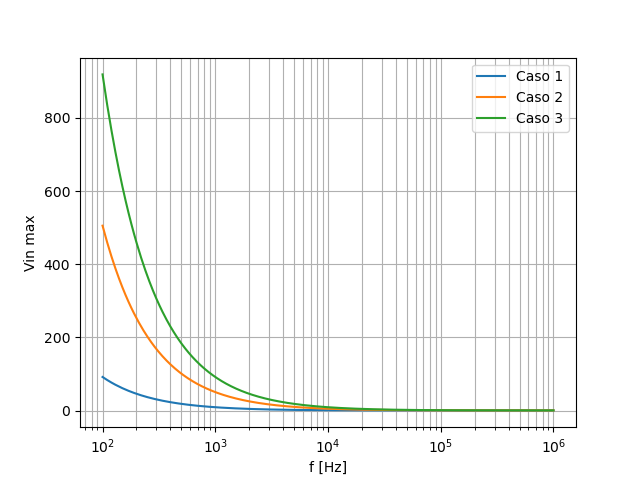
\includegraphics[width=.8\linewidth]{./Imagenes/SRNoInv.png}  
		\caption{Tensión de entrada limitada por efecto de Slew Rate}
	\end{subfigure}
	\caption{Circuito no inversor. Limitaciones a la tensión de entrada}
	\label{fig:invcasos}
\end{figure} 



Considerando ambos efectos, se puede obtener una aproximación teórica:

\begin{figure}[H]
	\centering
	\includegraphics[scale=0.5]{./Imagenes/NOInvVinMin.png}
	\caption{Limitaciones a la tensión de entrada por saturación y slew rate}
	\label{fig:circinvcaso1}
\end{figure}


Se siguió el mismo procedimiento descripto para el circuito inversor, utilizando el circuito empleado para medir la respuesta en frecuencia de la ganancia y la diferencia de fase. Superponiendo los datos medidos con los simulados y lo previsto por la teoría, se obtuvieron los siguientes gráficos:

\begin{figure}[H]
	\centering
	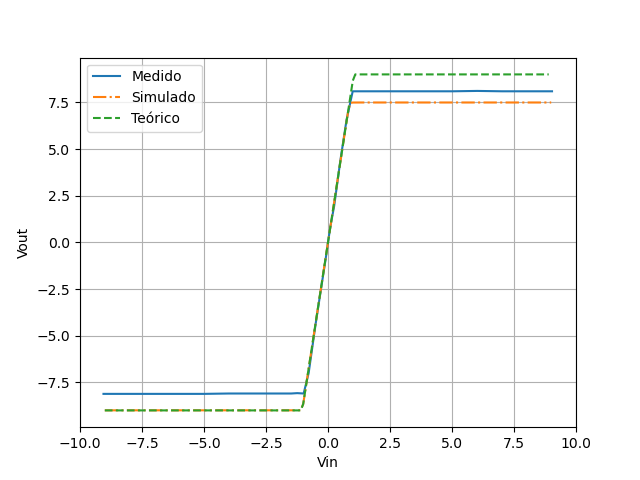
\includegraphics[scale=0.5]{./Imagenes/NoInvCaso1DC.png}
	\caption{DC Sweep: circuito no inversor caso 1}
	\label{fig:circinvcaso1}
\end{figure}

\begin{figure}[H]
	\centering
	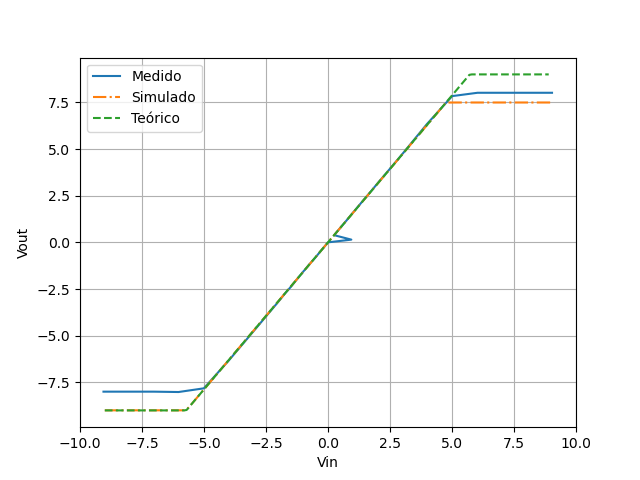
\includegraphics[scale=0.5]{./Imagenes/NoInvCaso2DC.png}
	\caption{DC Sweep: circuito no inversor caso 2}
	\label{fig:circinvcaso1}
\end{figure}

\begin{figure}[H]
	\centering
	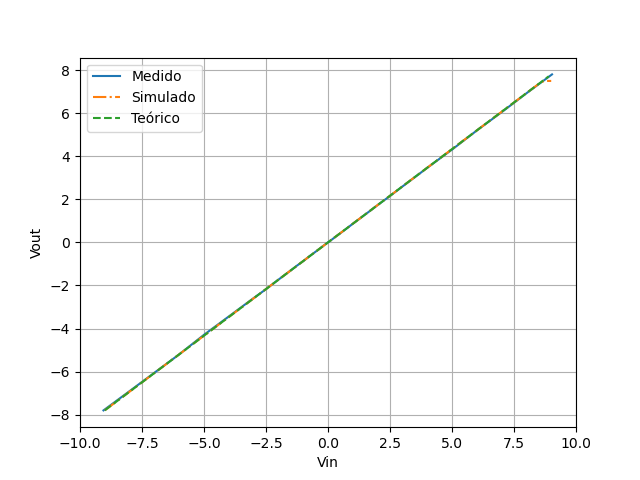
\includegraphics[scale=0.5]{./Imagenes/NoInvCaso3DC.png}
	\caption{DC Sweep: circuito no inversor caso 3}
	\label{fig:circinvcaso1}
\end{figure}

En los gráficos se verifica el comportamiento previsto por la teoría, aproximándose bastante bien con los datos simulados y medidos en la región del comportamiento lineal. Asimismo, se comprueba en la región lineal la ganancia en cada caso así como el carácter no inversor del circuito. Se observan las demás características descriptas anteriormente, tal como el valor de saturación, el cual resulta menor en módulo que $V_{cc}$, así como el rango de tensiones de entrada para el cual se mantiene la linealidad, el cual aumenta hacia el tercer caso. Es decir, un circuito de menor ganancia presenta un mayor rango de linealidad para la tensión de salida. 

En cuanto al efecto de \textbf{Slew Rate}, se siguió lo detallado arriba, con 
distintas configuraciones según cada caso. Se utilizó una señal senoidal de entrada de $2V_{pp}$ a una frecuencia de $500kHz$. Se utilizó el cursor para aproximar el SR, obteniendo distintos valores.

Se observan a continuación efectos del slew rate en los distintos casos del circuito no inversor.


\begin{figure}[H]
	\centering
	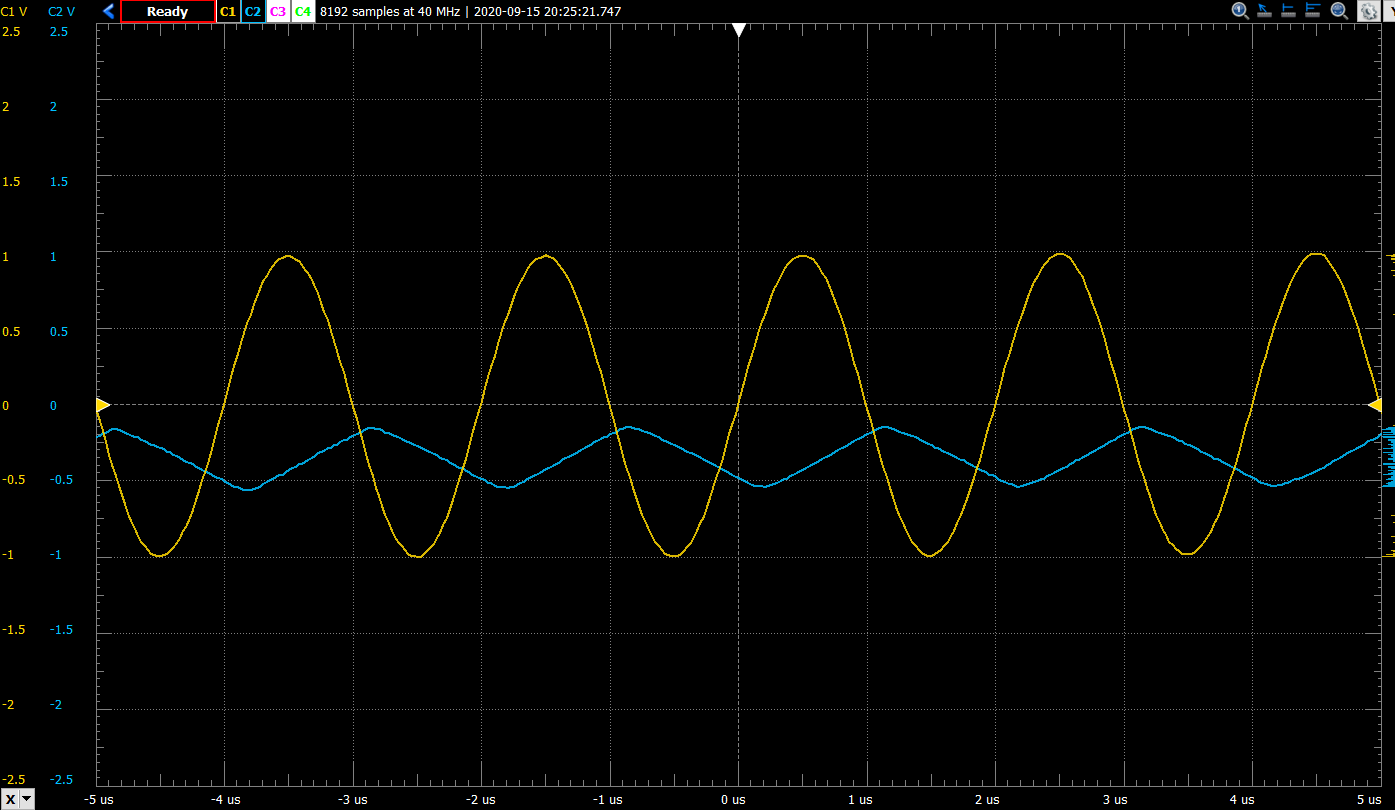
\includegraphics[scale=0.3]{./Imagenes/NoInvCaso1SR.png}
	\caption{Slew rate: señal de entrada a $500kHz$ y $2V_{pp}$. Caso 1.}
	\label{fig:circinvcaso1}
\end{figure}

\begin{figure}[H]
	\centering
	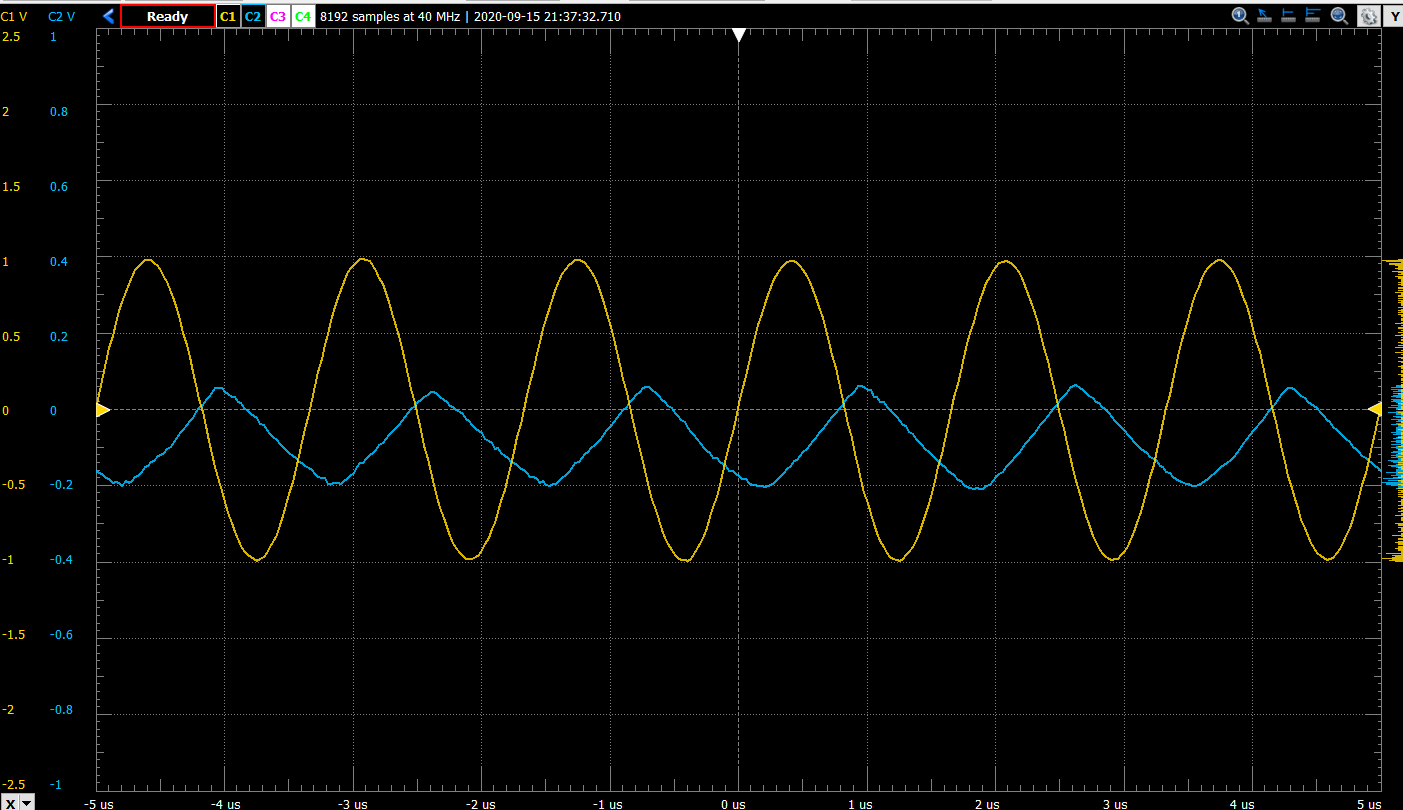
\includegraphics[scale=0.3]{./Imagenes/NoInvCaso2SR.png}
	\caption{Slew rate: señal de entrada a $500kHz$ y $2V_{pp}$. Caso 2.}
	\label{fig:circinvcaso1}
\end{figure}

\begin{figure}[H]
	\centering
	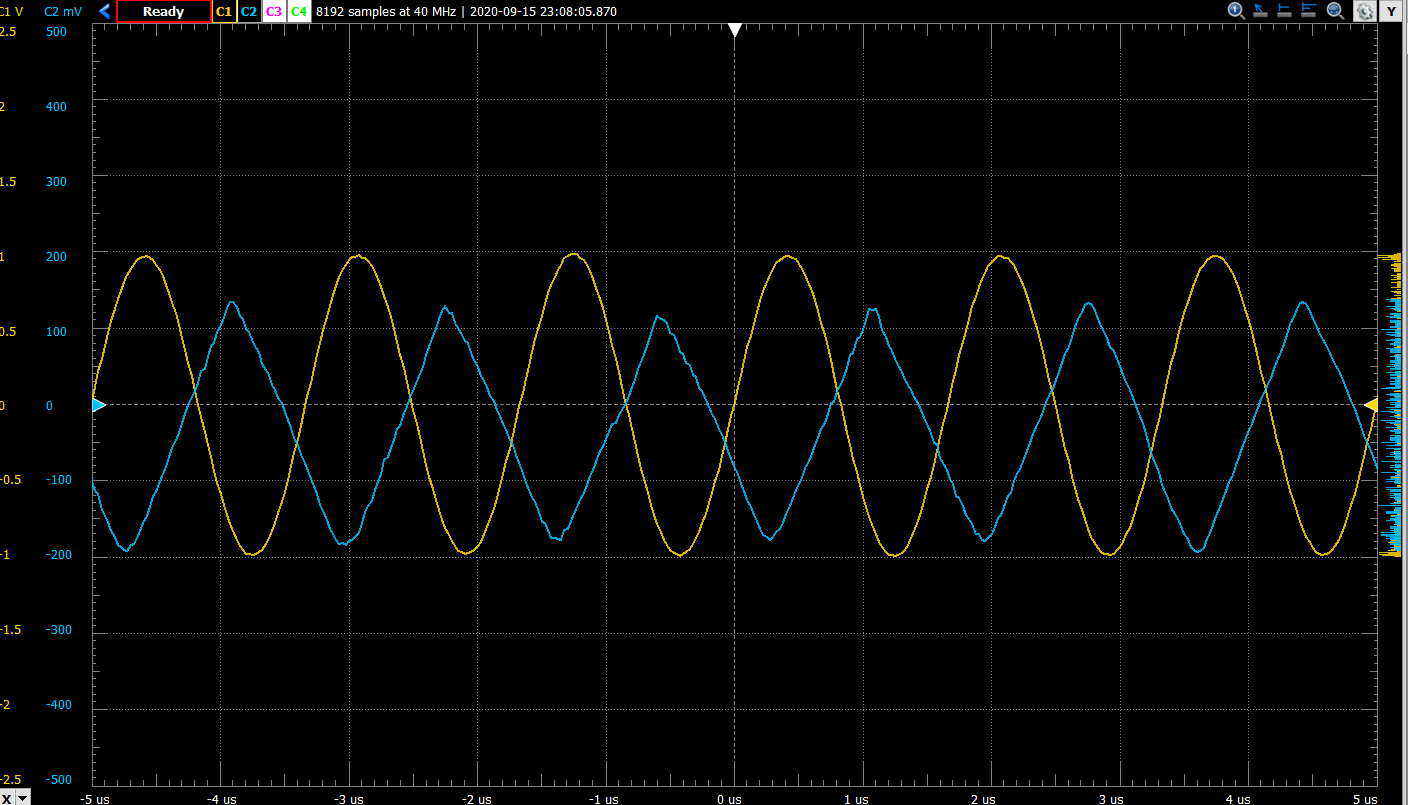
\includegraphics[scale=0.3]{./Imagenes/NoInvCaso3SR.png}
	\caption{Slew rate: señal de entrada a $500kHz$ y $2V_{pp}$. Caso 3.}
	\label{fig:circinvcaso1}
\end{figure}

